\documentclass[french]{article}
\usepackage{babel}
\usepackage[T1]{fontenc}
\usepackage[utf8]{inputenc}
\usepackage{lmodern}
\usepackage{times}
\usepackage{listings}
\usepackage{xcolor}
\usepackage{hyperref}
\usepackage{graphicx}

\definecolor{dkgreen}{rgb}{0,0.6,0}
\definecolor{bluebell}{rgb}{0.62,0.62,0.84}
\definecolor{mauve}{rgb}{0.58,0,0.82}

\lstset{frame=tb,
  language=Java,
  aboveskip=3mm,
  belowskip=3mm,
  showstringspaces=false,
  columns=flexible,
  basicstyle={\small\ttfamily},
  numbers=none,
  numberstyle=\tiny\color{purple},
  keywordstyle=\color{red},
  commentstyle=\color{bluebell},
  stringstyle=\color{mauve},
  breaklines=true,
  breakatwhitespace=true,
  literate={é}{{\'e}}1
  				 {ù}{{\`{u}}}1
  				 {â}{{\^{a}}}1
  				 {à}{{\`{a}}}1
  				 {è}{{\`e}}1,
  tabsize=3
}

\title{\vfill TP4 : Simulation de la propagation d'une maladie au sein d'une population}
\author{Jacques KOZIK, Arij HADDA et Killian GALFRE--VEYRET}
\date{Version du 06 avril 2024\vfill}

\begin{document}
\maketitle
\newpage

\tableofcontents
\newpage

\section{Introduction}

La modélisation de la propagation des maladies dans une population est un outil essentiel pour comprendre et gérer les épidémies. 

Les modèles multi-agents offrent une approche puissante pour simuler les interactions individuelles au sein d'une communauté et étudier l'émergence de phénomènes collectifs tels que la propagation d'une maladie infectieuse. Dans cette étude, nous développons un modèle multi-agent simple pour simuler la propagation d'une maladie au sein d'une population, en mettant en œuvre des mécanismes tels que l'infection, l'exposition, la récupération et la perte d'immunité.

Le modèle repose sur une grille en deux dimensions où chaque individu est caractérisé par son statut de santé, représenté par les états Susceptible (S), Exposé (E), Infecté (I) et Rétabli (R), ainsi que par les durées de vie associées à chaque état. Nous utilisons un espace toroïdal pour éviter les artefacts de bordure et permettre une interaction fluide entre les individus.

L'évolution de la maladie est modélisée sur une échelle de temps discrète, où chaque pas de temps correspond à un jour. Les individus se déplacent aléatoirement à chaque pas de temps, simulant ainsi les interactions spatiales au sein de la population. L'infection se produit lorsque des individus susceptibles entrent en contact avec des individus infectés dans leur voisinage, avec une probabilité calculée en fonction du nombre d'infectieux présents.

Nous intégrons également des mécanismes de transition d'état asynchrones, où les individus passent de l'état exposé à l'état infecté après une période d'exposition, puis de l'état infecté à l'état rétabli après une période infectieuse. De plus, nous prenons en compte la perte d'immunité avec le temps, où les individus rétablis peuvent redevenir susceptibles après une période donnée.

En initialisant la simulation avec un nombre spécifique d'individus dans chaque état de santé et en définissant les paramètres de durée de vie de manière aléatoire, nous examinons comment différents scénarios affectent la dynamique de la maladie au fil du temps.

Dans cette étude, nous présentons le cadre général de notre modèle multi-agent de propagation de la maladie et discutons de son application potentielle pour comprendre et prévoir les épidémies dans des contextes réels.

\section{Description du modèle}

Pour mettre en œuvre cette simulation, nous avons opté pour une approche combinant des classes Java avec l'utilisation du générateur Mersenne Twister. Et pour le rendu, nous avons inscrits nos résultats dans des fichiers CSV puis avons, à l'aide d'un notebook Jupyter, généré des graphiques pour les illustrer.

\subsection{Générateur Mersenne Twister (MTrandom)} \label{sec/MT}

Le générateur Mersenne Twister, largement utilisé en Java pour la génération de nombres aléatoires, est apprécié pour sa haute qualité et sa performance. En Java, il est implémenté sous forme de classe, offrant une interface simple et efficace pour la génération de nombres aléatoires. Cette méthode de génération de nombres aléatoires est basée sur un algorithme développé par Matsumoto et Nishimura, qui produit des séquences de nombres pseudo-aléatoires présentant d'excellentes propriétés statistiques. En utilisant le générateur Mersenne Twister en Java, les développeurs peuvent facilement introduire des éléments de stochasticité dans leurs simulations, ce qui est crucial pour modéliser des phénomènes complexes tels que la propagation des maladies dans une population. La robustesse et la fiabilité de Mersenne Twister en font un choix populaire pour de nombreuses applications nécessitant une génération de nombres aléatoires de haute qualité en Java.

Nous avons également ajouter une méthode negExp dans la classe MTrandom, qui prend en paramètre un réel mean, et qui renvoie un réel entre 0 et mean.

\begin{lstlisting}
	/*method negExp, qui genere un nombre entre 0 et inMean*/
	public double negExp(double inMean) {
        return -inMean * Math.log(1 - this.nextDouble());
    }
\end{lstlisting} 

\subsection{Implémentation de Classes}

\subsubsection{Humain}
Pour commencer, nous avons décider de créer une classe Humain, avec comme attributs un statut (statut) sous forme de caractère, un entier temps (temps), un entier de durée de temps exposés (dE), un entier de durée de temps infectés (dI) et enfin un entier de durée de temps de récupération (dR).

On peut créer la classe avec le code suivant:

\begin{lstlisting}

public class Humain {
    private char statut;
    private int temps;
    private int dE;
    private int dI;
    private int dR;
    private MTRandom random = new MTRandom();

    //Constructeur

    public Humain(char s){
        statutValide(s);
        this.statut=s;
        this.temps=0;
        this.generate_dE();
        this.generate_dI();
        this.generate_dR();
    }


    private void statutValide(char s){
        if ((s!='S')&&(s!='E')&&(s!='I')&&(s!='R')){
            throw new IllegalArgumentException("statut non valide");
        }
    }


	//Setteurs
	
    public void SetStatut(char s){
        statutValide(s);
        this.statut=s;
    }

    public void SetTemps(int n){
        this.temps = n;
    }

    public void generate_dE(){
        this.dE = (int) random.negExp(3);
        
    }

    public void generate_dI(){
        this.dI = (int) random.negExp(7);
        
    }

    public void generate_dR(){
        this.dR = (int) random.negExp(365);
    }
    
}

\end{lstlisting}
Les méthodes generate\_dE, generate\_dI et generate\_dR permettent de générer des durées de temps exposés, de temps infectés et de récupération respectivement avec l'aide de la méthode negExp de la classe MTrandom.

Nous avons également des Getteurs pour récupérer la valeur des attributs privé :

\begin{lstlisting}
    //Getteurs

    public char GetStatut(){
        return this.statut;
    }
    public int GetTemps(){
        return this.temps;
    }
    public int GetdE(){
        return this.dE;
    }
    public int GetdI(){
        return this.dI;
    }
    public int GetdR(){
        return this.dR;
    }
\end{lstlisting}

\subsubsection{GrilleHumain}

Suite à cela, nous avons opté pour la création d'une classe appelée `GrilleHumain`. Son objectif est de générer des instances représentant une grille toroïdale, où chaque case peut contenir une liste d'humains. Plusieurs humains distincts peuvent se trouver sur une même case.
On peut la créer avec le code suivant:
\begin{lstlisting}
import java.io.FileWriter;
import java.io.IOException;
import java.io.PrintWriter;
import java.util.ArrayList;
import java.util.List;


public class grilleHumain {
    // Attributs
    private ArrayList<Humain>[][] grille;
    public static MTRandom random = new MTRandom();

    // Constructeur

    /* grilleHumain, methode de contruction de la classe grilleHumain qui creer un tableau a deux dimensions,
     * et qui place un tableau ou peuvent etre placer des objets de classe Humain dans chaque case. */

    @SuppressWarnings("unchecked")
    public grilleHumain(int lignes, int colonnes) {
        this.grille = new ArrayList[lignes][colonnes];
        for (int i = 0; i < lignes; i++) {
            initialiserLigne(i, colonnes);
        }
    }

    /* InitialiserLigne, methode utiliser dans le constructeur pour initialiser les lignes du tableau. */

    private void initialiserLigne(int ligne, int colonnes) {
        for (int j = 0; j < colonnes; j++) {
            grille[ligne][j] = new ArrayList<Humain>();
        }
    }
\end{lstlisting}

Nous avons ensuite créer deux méthodes permettant de remplir cette grile avec un nombre n d'individus. La première, addHumain() prend en paramètre un humain et le place de manière aléatoire sur une case de la grille. Pour cela, elle fait appel à la fonction negExp() qui génère un nombre compris entre 0 et la taille de la grille (300 dans notre cas) en se basant sur le générateur de nombre de Mersenne Twister (cf. section \ref{sec/MT}). Une seconde, addAllHumains(), qui se charge de créer les humains qui doivent être positionnés sur la grille puis qui fait appel à la fonction susmentionné pour le faire.

\lstinputlisting[language=Java, firstline=36, lastline=54]{grilleHumain.java}

Dans un troisième temps, nous avons créés les méthodes permettant de calculer le nombre d'humains inféctés par rapport à une case donnée. Il y en a 3, la première récupère une liste d'humain (il y en a une dans chaque case). La seconde, compte le nombre d'humain dont le statut et 'I' (pour Infected) dans la case et la troisième fait répéter ce comptage sur les 8 cases autour.

\lstinputlisting[language=Java, firstline=74, lastline=112]{grilleHumain.java}

\noindent Puis ensuite les dernières méthodes créées servent à mettre en place la simulation :

\begin{description} \label{liste/descMéthode}
\item[checkEtat] Regarde l'état d'un humain et met en place la conduite défini dans le sujet (eg. pour un infécté, on regarde d'abord si le temps depuis lequel il est dans cet état, est supérieur au temps pendant lequel il doit y rester - défini aléatoirement - puis si c'est le cas, alors on lui change son statut pour le suivant, sinon, on incrémente le temps passé dans ce statut de +1)
\item[deplacementHumains] Déplace tout les humain sur une autre case quelle qu'elle soit et de manière aléatoire.
\item[simulation] Lance la simulation et écrit au fur et à mesure, le nombre d'humain dans chaque état dans un fichier CSV. Pour cela, elle crée d'abord 19 980 humains dans l'état Susceptible et 20 dans l'état Infecté. Ensuite, elle lance une boucle de 730 itérations, qui correspond à 730 jours. A l'intérieur, pour chaque humain, on appel la fonction checkEtat() puis ensuite on incrémente en fonction de son nouvel état, les variables permettant de compter le nombre d'individu dans chaque état. Une fois fait pour tout les individus, on appel la fonction deplacementHumains() puis on inscrit les résultats des variables compteur dans le CSV. ET on recommence 729 fois !
\end{description}

\lstinputlisting[language=Java, firstline=115, lastline=224]{grilleHumain.java}

\subsubsection{Main}
Cette classe, qui se veut la plus simple et courte possible, permet le lancement du programme. Pour cela, elle crée une méthode \textit{main} qui, à travers une boucle for, éxecute 100 fois les 2 commandes suivante : création d'une grille vide puis lancement de la simulation par l'appel de la fonction simulation() qui gère toute la simulation (cf. section \ref{liste/descMéthode}).

\lstinputlisting[language=Java, firstline=1, lastline=9]{Main.java}

\section{Résultats}
En réalisant la simulation 100 fois, on obtient toujours des résultats proche les uns des autres. Voici le graphe obtenu lors de notre 50-ième itération. \newline
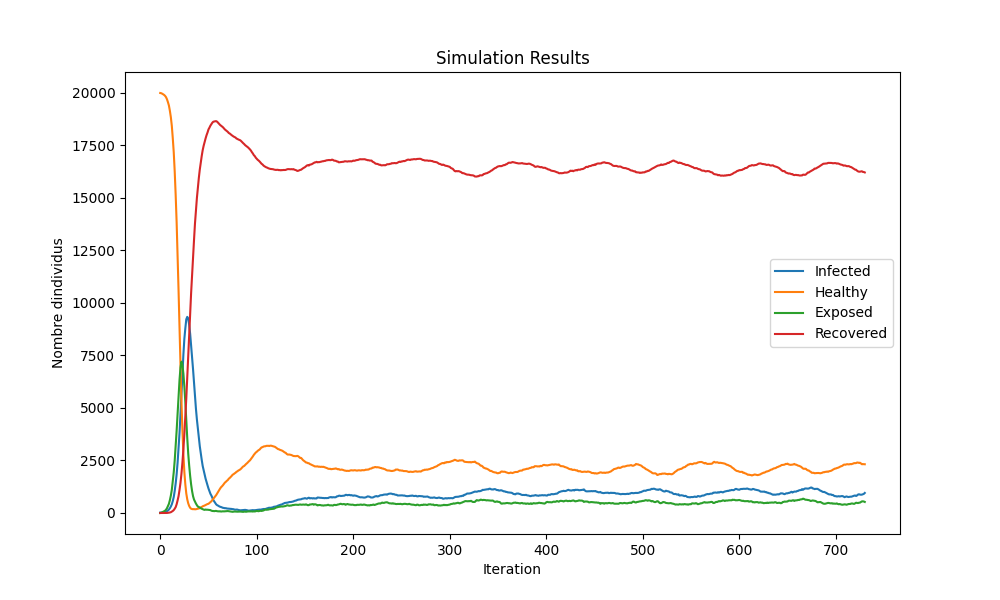
\includegraphics[scale=0.5]{./simulation_results_png/simulation_results_50.png} On constate - à chaque fois - que le pique d'exposé est atteint entre le 25-ième jour et le 30-ième. Le pique des infectés suit logiquement quelques jours après, autour du 30-ième jour. Puis celui des 'Recovered' encore après. Autour du 55-ième jour. A l'inverse, le nombre de 'Susceptible' chute en même temps que celui de 'Exposed' et 'Infected' augmente, soit autour du 30-ième jour. Il reste ensuite très faible puisque les personnes ayant le status 'Recovered' ne peuvent pas être réinfectés pendant un certain temps.

\section{Conclusion}
La modélisation de la propagation des maladies dans une population est cruciale pour comprendre les épidémies. A travers ce projet, nous avons développé un modèle multi-agent permettant de simuler la propagation d'une maladie au sein d'une population, en mettant en œuvre des mécanismes tels que l'exposition, l'infection, la récupération et la perte d'immunité. En utilisant une approche basée sur des classes Java et le générateur Mersenne Twister, nous avons pu créer un modèle robuste et flexible. Et à l'aide d'un notebook Jupyter nous avons pu réaliser des graphiques pour étudier les résultats de nos simulations.

Notre étude a donc révélé des résultats cohérents, avec des simulations répétées montrant des schémas similaires dans la dynamique de la maladie. Le pic d'exposition est généralement observé entre le 25e et le 30e jour, suivi du pic des infectés quelques jours plus tard, et enfin du pic des personnes récupérées. De plus, nous avons constaté une diminution significative du nombre de personnes susceptibles après le pic d'infections, témoignant de l'acquisition d'une immunité partielle au sein de la population.

Ces résultats démontrent l'efficacité de notre modèle pour simuler la propagation des maladies et pour comprendre les tendances épidémiologiques. En combinant des techniques de modélisation multi-agent avec des outils de programmation robustes, notre approche offre un cadre précieux pour étudier et prévoir les épidémies dans des contextes réels.
\end{document}